%! Author = karen
%! Date = 2/18/2024

% Preamble
\documentclass[11pt]{article}

% Packages
\usepackage{amsmath}
\usepackage{graphicx}
\usepackage{amssymb}




\author{Karen Dianelis Cantero Lopez C411 \\ Loitzel Ernesto Morales Santiesteban C412}
\title{Proyecto 1. \\ Simulación \\ Cola con n servidores en paralelo}


% Document
\begin{document}

    \maketitle
    \newpage

    \tableofcontents
    \newpage

    \section{Introducción}
    En este proyecto pretendemos simular el comportamiento de una cola ante un servicio que posee n servidores en paralelo. Cuando un cliente llega, se une a la cola si todos los servidores están ocupados. Si algún servidor está libre, el cliente entrará al primer servidor (del 1 al n) que esté libre.
    Cuando un cliente completa el servicio con un servidor (no importa cuál), ese cliente luego abandona el sistema. El cliente que ha estado en la cola durante más tiempo (si hay clientes en la cola) entra en servicio.



    \subsection{Objetivos y Metas}
    El objetivo principal del proyecto es simular el sistema descrito anteriormente para comprender su comportamiento y desempeño bajo diferentes condiciones y distribuciones de arribos y servicio. Las metas específicas incluyen:

    \begin{itemize}
\item Analizar el tiempo de espera promedio de los clientes en la cola para evaluar la eficiencia del sistema en la atención de los clientes.
\item Determinar el tiempo de espera máximo experimentado por un cliente en la cola para identificar posibles casos extremos de espera.
\item Calcular la cantidad total de clientes atendidos durante la simulación para entender la capacidad de procesamiento del sistema.
\item Estimar la cantidad de clientes que no se llegan a atender debido a la falta de capacidad del sistema.
\item Evaluar la probabilidad de que un cliente no pueda ser atentido inmediatamente debido a la falta de capacidad del sistema (probabilidad de que el sistema esté saturado) para comprender la eficiencia del sistema en la gestión de la demanda y la asignación de recursos.
\item Estimar el tiempo promedio que un cliente en el sistema (en la cola y en el servidor)
\item Calcular la probabilidad de que el sistema tenga 0 clientes para poder determinar la eficiencia y capacidad del sistema.
    \end{itemize}

    \subsection{Variables que describen el problema}

    \begin{itemize}
        \item Cantidad de servidores: Representa el número de servidores disponibles en el sistema para atender a los clientes.

        \item Tiempo de servicio: Indica la duración total del servicio.

        \item Distribución de llegada de clientes: Describe el patrón o la ley que sigue la llegada de nuevos clientes al sistema.

        \item Distribución de tiempo de servicio: Indica cómo se distribuyen los tiempos de servicio de los servidores al atender a los clientes.

        \end{itemize}



    \section{Sistema Específico y Variables de Interés}
    \subsection{Sistema Específico}
    Como ya se ha dicho en la introducción, el sistema que se va a simular
es un sistema con n servidores en paralelo. Cada servidor puede seguir una distribución distinta del tiempo de atención.
El tiempo de llegada de los clientes también puede seguir una distribución distinta.

Para facilitar el uso de nuestra implementación, se han dejado ya implementadas las distribuciones de poisson, exponencial, normal y uniforme.


    \subsection{Variables de Interés}
    Las variables de interés en este problema son:
    \begin{itemize}
        \item Tiempo de espera promedio de los clientes en la cola: Representa el tiempo promedio que un cliente pasa esperando en la cola antes de ser atendido.

\item Promedio del tiempo de espera máximo experimentado por un cliente en la cola: Este valor ayuda a identificar casos extremos de espera.

\item Promedio de la cantidad total de clientes atendidos durante la simulación: Representa el número total de clientes que han sido atendidos y han completado su servicio en el sistema durante la simulación.

\item Promedio de la cantidad de clientes que no se llegan a atender debido a la falta de capacidad del sistema: Es una indicación de la capacidad del sistema.

\item Probabilidad de que un cliente no pueda ser atendido inmediatamente debido a la falta de capacidad del sistema: Esta probabilidad es una medida de la eficacia del sistema en la gestión de la demanda y la asignación de recursos.

    \end{itemize}

    \section{Detalles de Implementación}
    \subsection{Lenguaje de Programación}
    Para la implementación de la simulación se utilizó el lenguaje de programación Python.

    \subsection{Pasos seguidos para la implementación}
    Los pasos seguidos para la implementación de la simulación fueron:
    \begin{itemize}
        \item Modelar distintos tipos de distribuciones.
        \item Crear las clases StatisticsHolder, StateVariables y Sim para mantener una estructura limpia en el código.
        \item Implementar el algoritmo de simulación teniendo en cuenta las diferentes distribuciones y almacenando los datos necesarios para el análisis.
        \item Realizar pruebas de los modelos implementados y comparar con los resultados matemáticos.
    \end{itemize}

    \section{Resultados y Experimentos}

    \subsection{Hallazgos de la simulación}

    Para poder comparar como afecta cada parámetro a los resultados de la simulación, simularemos 4 escenarios distintos,
    en cada uno variando solo una variable. 
    
    Para todas las simulaciones mantendremos constante la distribución Poisson como distribución de llegada a la cola (por lo tanto los tiempos entre las llegadas
    distribuyen de forma exponencial) y la distribución Poisson como distribución de los tiempos de atención en los servidores ya que estos tiempos también son de forma exponencial.\\
    $\lambda$ va a representar el parámetro de la distribución de llegada de clientes, $\mu$ va a representar el parámetro
    de la distribución de los tiempos de atención, y $n$ representará la cantidad de servidores.

    
    \subsubsection{Simulación 1}

    Usaremos:
    \begin{itemize}
        \item $\lambda$ = 2
        \item $\mu $= 1
        \item $n$ = 3
    \end{itemize}

    Obtuvimos estos resultados: \\

    \begin{table}[h]
\begin{tabular}{|l|l|l|l|}
\hline
\textbf{variable}                                 & \textbf{media} & \textbf{varianza} & \textbf{desviación estándar} \\ \hline
\textit{probabilidad de encolarse}                & 0.44           & 0.001             & 0.001                         \\ \hline
\textit{probabilidad de 0 clientes en el sistema} & 0.11           & 0.0001            & 0.0003                        \\ \hline
\textit{Longitud promedio de la cola}             & 425            & 3268              & 1.8                           \\ \hline
\textit{Tiempo promedio en cola}                  & 0.43           & 0.009             & 0.003                         \\ \hline
\textit{Tiempo promedio en el sistema}            & 1.43           & 0.01              & 0.003                         \\ \hline
\end{tabular}
\end{table} 

    \subsubsection{Simulación 2}

    Ahora probaremos con las mismas variables, solo cambiando $\lambda = 4$ 
    \begin{itemize}
        \item $\lambda$ = 4
        \item $\mu$ = 1
        \item $n$ = 3
    \end{itemize} 

    \begin{table}[h]
\begin{tabular}{|l|l|l|l|}
\hline
\textbf{variable}                                 & \textbf{media} & \textbf{varianza} & \textbf{desviación estándadr} \\ \hline
\textit{probabilidad de encolarse}                & 0.99          & 0.000002             & 0.000049                    \\ \hline
\textit{probabilidad de 0 clientes en el sistema} & 0.0009         & 0.0000007            & 0.000014                        \\ \hline
\textit{Longitud promedio de la cola}             & 1913            & 2043              & 1.42                           \\ \hline
\textit{Tiempo promedio en cola}                  & 59.85           & 54.42            & 0.34                       \\ \hline
\textit{Tiempo promedio en el sistema}            & 60.59           & 54.29             & 0.23                      \\ \hline
\end{tabular}
\end{table}

    \newpage
\subsubsection{Simulación 3}
    Ahora probaremos con las mismas variables, solo cambiando $\mu = 4$ \\
    \begin{itemize}
        \item $\lambda$ = 2
        \item $\mu$ = 4
        \item $n$ = 3
    \end{itemize}

    \begin{table}[h]
\begin{tabular}{|l|l|l|l|}
\hline
\textbf{variable}                                 & \textbf{media} & \textbf{varianza} & \textbf{desviación estándar} \\ \hline
\textit{probabilidad de encolarse}                & 0.015          & 0.000031             & 0.00017                    \\ \hline
\textit{probabilidad de 0 clientes en el sistema} & 0.60          & 0.00021            & 0.00046                        \\ \hline
\textit{Longitud promedio de la cola}             & 14.68            & 30.40              & 0.17                         \\ \hline
\textit{Tiempo promedio en cola}                  & 0.0015           & 0.00000084            & 0.000029                     \\ \hline
\textit{Tiempo promedio en el sistema}            & 0.2513           & 0.000073             & 0.00027                      \\ \hline
\end{tabular}
\end{table} 

    \subsubsection{Simulación 4}
    Ahora probaremos con las mismas variables, solo cambiando $ n = 8$ \\
    Usaremos:
    \begin{itemize}
        \item $\lambda$ = 2
        \item $\mu $= 1
        \item $n$ = 8
    \end{itemize}

\begin{table}[h]
\begin{tabular}{|l|l|l|l|}
\hline
\textbf{variable}                                 & \textbf{media} & \textbf{varianza} & \textbf{desviación estándar} \\ \hline
\textit{probabilidad de encolarse}                & 0.001          & 0.0.0000028             & 0.000043                    \\ \hline
\textit{probabilidad de 0 clientes en el sistema} & 0.13          & 0.00027            & 0.0005                        \\ \hline
\textit{Longitud promedio de la cola}             & 1.098            & 2.72              & 0.05                         \\ \hline
\textit{Tiempo promedio en cola}                  & 0.0002          & 0.00000018            & 0.000013                     \\ \hline
\textit{Tiempo promedio en el sistema}            & 0.999           & 0.0010             & 0.001                     \\ \hline
\end{tabular}
\end{table}



    \subsection{Interpretación de los resultados}

    Tomaremos los resultados de la simulación 1 como base para comparar cómo el cambiar los parámetros afecta los resultados.

    \subsubsection{Variando el valor $\lambda$}
    Podemos apreciar que al aumentar el valor de $\lambda$ y mantener todos los demás valores igual :
    \begin{itemize}
        \item La cantidad de personas encoladas aumentan, ya que la cantidad de personas en el sistema aumenta, debido a que lambda simboliza la cantidad de personas que llegan en un tiempo t.
        \item Los tiempos promedio que una persona permanece en la cola, y por ende en el sistema, aumentan.
        \item Al aumentar el flujo de personas, la probabilidad de encolarse aumenta, y la probabilidad de que el sistema esté vacío disminuye.
    \end{itemize}

    \subsubsection{Variando el valor $\mu$}
    Podemos apreciar que al aumentar el valor de $\mu$ y mantener todos los demás valores igual :
    \begin{itemize}
        \item La cantidad de personas encoladas disminuyen, ya que los tiempos de atención de los servidores disminuyen porque los servidores pueden soportar una carga mayor (esto es lo que $\mu$ representa en este caso)
        \item Los tiempos promedio que una persona permanece en la cola, y por ende en el sistema, disminuyen.
        \item Al disminuir el tiempo de atención, la probabilidad de encolarse disminuye, y la probabilidad de que el sistema esté vacío aumenta.
    \end{itemize}

    \subsubsection{Variando el valor $n$}
    Podemos apreciar que al aumentar el valor de $n$ y mantener todos los demás valores igual :
     \begin{itemize}
        \item La cantidad de personas encoladas disminuyen, ya que ahora existen más servidores disponibles para atender a los clientes.
        \item La probabilidad de encolarse también disminuye notablemente ya que existen más servidores disponibles.
         \item El tiempo promedio en la cola disminuye notablemente ya que existen más servidores disponibles.
         \item El tiempo promedio en el sistema no cambia notablemente con respecto a la Simulación 1 ya que no hemos variado el valor de $\mu$ que influye en el el tiempo de atención.
    \end{itemize}

    \subsubsection{Alta varianza en resultados}
    Una alta varianza en los resultados nos dice que los valores varían notablemente entre las simulaciones.\\
    En nuestras simulaciones, la varianza es alta en la cantidad de clientes en el sistema y en la longitud promedio de la cola. 
    Esto nos dice que el sistema es muy sensible a cambios en los parámetros, y que los resultados pueden variar mucho entre simulaciones.\\


    \subsection{Necesidad de realizar el análisis estadístico a la simulación}
    El análisis estadístico de los resultados de una simulación es fundamental para comprender y extraer información
    relevante de los datos generados por la simulación.

    Este análisis permite evaluar la precisión del modelo de simulación, y ayuda
    a identificar posibles problemas o limitaciones en el modelo. Además, proporciona una base para
    la toma de decisiones informadas y la identificación de áreas de mejora en el sistema simulado.

    Nosotros hemos analizado la media, la varianza, la desviacón estándar y el percentil 95 de las variables que identificamos
    como de interés en la sección 2.2. Un ejemplo de este análisis se muestra más adelante en la sección 5.2.1


    \subsection{Análisis de parada de la simulación}
    En nuestra simulación, se establecieron dos criterios de parada principales para determinar el momento adecuado para finalizar las corridas:

    \begin{itemize}
    \item Desviación estándar: Buscábamos una desviación estándar pequeña en los resultados de las simulaciones. La desviación estándar mide la dispersión de los datos alrededor de la media, por lo que buscamos un valor bajo (menor al 10\% de la media) lo cual indica que los resultados son consistentes y confiables.

    \item Número de simulaciones: Se ejecutó un gran número de simulaciones para obtener un conjunto de datos robusto y minimizar el impacto de la aleatoriedad inherente a las simulaciones.
    \end{itemize}

    \subsection{Validación con el modelo matemático:}

    Para corroborar la precisión de la simulación, se compararon los resultados con los valores obtenidos mediante el modelo matemático correspondiente. Esta comparación permitió verificar que la simulación se comporta como se esperaba, siguiendo las predicciones del modelo teórico.




    \section{Modelo Matemático}
    \subsection{Descripción del modelo de la simulación}
    En esta simulación, modelamos una cola M/M/c o de Erlang. \\
- M: Indica que las llegadas de clientes siguen una distribución de Poisson (M), lo que significa que los intervalos de tiempo entre las llegadas sucesivas de clientes siguen una distribución exponencial.\\
- M: También indica que los tiempos de servicio en el sistema siguen una distribución exponencial, lo que significa que la duración del servicio para cada cliente es independiente y sigue una distribución exponencial.\\
- c: Representa el número de servidores en el sistema. En el sistema M/M/c, hay múltiples servidores disponibles para atender a los clientes que llegan a la cola.\\
El tamaño de la cola es infinito, lo que significa que no hay límite para la cantidad de clientes que pueden esperar en la cola.

Usamos estas distribuciones ya que en la literatura se ha demostrado que son las más adecuadas para modelar sistemas de colas, y podremos usar los resultados de la teoría de cola para comparar con los resultados obtenidos en la simulación.

    \subsection{Comparación con la teoría de colas}
    Este modelo se compara con la teoría de colas para validar los resultados obtenidos. La
    teoría de colas nos proporciona fórmulas y ecuaciones para calcular y predecir el comportamiento de los sistemas de colas.


    \begin{itemize}
        \item $\rho$ = $\lambda$ / (c$\mu$) representa la utilización promedio del sistema, que es la fracción de tiempo que los servidores están ocupados. Si rho es mayor que 1, el sistema está sobrecargado y no puede manejar la tasa de llegada de clientes. Las métricas solo son confiables si $\rho < 1$.
        \item c: representa el número de servidores en el sistema.
        \item $\lambda$: representa la tasa de llegada promedio de los clientes al sistema siguiendo una distribución de Poisson.
        \item $\mu$: representa la tasa de servicio promedio de los servidores en el sistema siguiendo una distribución exponencial.
    \end{itemize}

    Se utilizaron las siguientes fórmulas matemáticas para comparar con los resultados obtenidos en la simulación:
    \begin{itemize}
        \item Probabilidad de que el cliente tenga que esperar en la cola: La probabilidad de que un cliente tenga que esperar en la cola se puede calcular utilizando la fórmula de Erlang C, que se define como:
        $$ C(c, p) = \frac{1}{1 +  (1 - p) (\frac{c!}{(cp)^c}) (\sum_{k=0}^{c-1} \frac{cp^k}{k!}) } $$
        \item Cantidad promedio de clientes en el sistema: La cantidad promedio de clientes en el sistema se puede calcular utilizando la fórmula conocida como de Little:
        $$ L_s = \lambda W_s$$
        \item Probabilidad de que el sistema tenga 0 clientes: La probabilidad de que el sistema tenga 0 clientes se puede calcular utilizando la fórmula:
        $$ P_0 = \frac{1}{\sum_{m=0}^{c-1} \frac{(c\rho)^m}{m!} + \frac{(c\rho)^c}{c!(1-\rho)}}$$
        \item Cantidad promedio de clientes en la cola: La cantidad promedio de clientes en la cola se puede calcular utilizando la fórmula:
        $$ L_q = \frac{P_0(\frac{\lambda}{\mu})^c\rho}{c!(1-\rho)^2} $$
        \item Tiempo promedio que un cliente pasa en la cola: El tiempo promedio que un cliente pasa en la cola se puede calcular utilizando la fórmula:
        $$ W_q = \frac{L_q}{\lambda} $$
        \item Tiempo promedio que un cliente pasa en el sistema: El tiempo promedio que un cliente pasa en el sistema se puede calcular utilizando la fórmula:
        $$ W_s = W_q + \frac{1}{\mu} $$

    \end{itemize}

    \subsubsection{Comparación}

    A continuación presentamos los resultados obtenidos de 3 simulaciones acompañados de los resultados que la teoría predice.

    \begin{table}[h]
\begin{tabular}{|l|ll|ll|ll|}
\hline
Valores                                  & \multicolumn{2}{l|}{$\lambda$ = 2, $\mu$=1, $c$=8}      & \multicolumn{2}{l|}{$\lambda$ = 3, $\mu$=3, $c$=4}       & \multicolumn{2}{l|}{$\lambda$ = 1, $\mu$=2, $c$=4}      \\ \hline
                                         & \multicolumn{1}{l|}{Obtenido} & Aprox. & \multicolumn{1}{l|}{Obtenido} & Aprox. & \multicolumn{1}{l|}{Obtenido} & Aprox. \\ \hline
Prob. de encolarse                       & 0.0011                                  & 0.0011       & 0.02                                    & 0.02         & 0.0018                                  & 0.0018       \\ \cline{1-1}
Cant. de clientes                     & 960.52                                  & 960.18       & 1438.47                                 & 483.26       & 480.911                                 & 240.12       \\ \cline{1-1}
Prob. 0 clientes                         & 0.1366                                  & 0.1353       & 0.3676                                  & 0.3673       & 0.6081                                  & 0.6064       \\ \cline{1-1}
Longitud de cola                & 1.139                                   & 0.1833       & 29.101                                  & 3.2653       & 0.882                                   & 0.1237       \\ \cline{1-1}
Tiempo en cola                  & 0.00019                                 & 0.00019      & 0.0022                                  & 0.0022       & 0.00027                                 & 0.00025      \\ \cline{1-1}
Tiempo en sistema               & 0.9986                                  & 1.0001       & 0.3357                                  & 0.3356       & 0.5001                                  & 0.5002       \\ \hline
\end{tabular}
\end{table}

[20pt]

    Ejemplo de análisis estadístico que realizamos a las variables:

    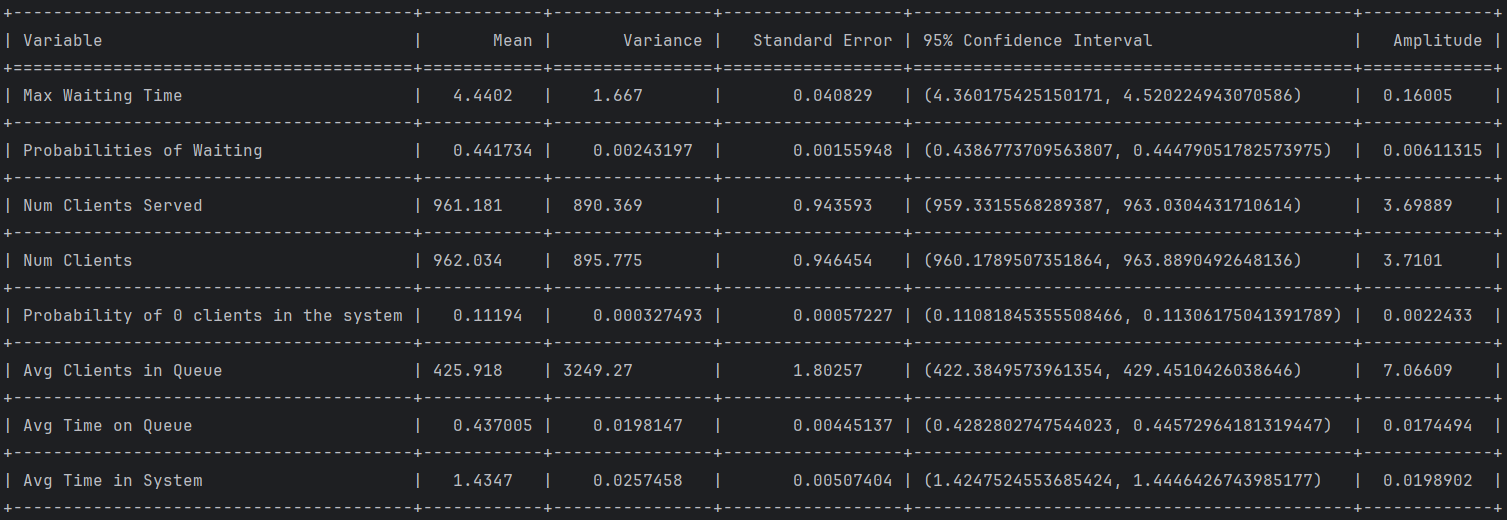
\includegraphics[width=1\textwidth]{images/8} \\

    Como se puede observar, la mayoría de los resultados son consistentes con los resultados teóricos. Esto indica que el modelo
    de simulación implementado es preciso y puede utilizarse para aproximar el comportamiento y el rendimiento del sistema M/M/c.


    \subsection{Supuestos y Restricciones}
    Los supuestos y restricciones del modelo son:
    \begin{itemize}
       \item Movimiento instantáneo entre servidores: Se asume que el movimiento de clientes entre servidores es instantáneo, lo que significa que un cliente puede pasar de un servidor a otro sin demora alguna.

\item Distribución invariable de llegadas de clientes: Se supone que la distribución de llegadas de clientes no cambia con el tiempo. Esto implica que la tasa de llegada de clientes se mantiene constante durante toda la simulación.

\item Permanencia de clientes no atendidos: Se establece que un cliente que llega al sistema permanece en el sistema hasta que es atendido por un servidor o hasta que concluye el tiempo de servicio sin ser atendido. No se permite que un cliente abandone el sistema sin ser atendido, a menos que expire el tiempo de servicio.


    \end{itemize}




\end{document}